In the previous chapters, we proposed and analyzed multiqubit gates based on resonant driving, and found that the gate times increased rapidly as the number of qubits $n$ grew. In this chapter, we take on the ambitious task to construct resonant gates that are efficient for larger system sizes, even beating optimal circuit decompositions of such gates. 

In \cref{sec:gatesintrointro}, we describe that the best known decomposition of the \texttt{Toffoli}$_n$ gate requires a circuit of depth $O(\log(n))$, which involves $O(n)$ ancillary qubits. Is there any hope that a continuous evolution can implement the same gate, such that the gate time $T$ grows \emph{slower} than logarithmically in $n$? We investigate this question by coupling $n$ qubits to a single ancilla. Straightforwardly simulating the resulting evolution using the the Trotter-Suzuki formula \cite{Lloyd1996} would result in a circuit of depth $O(n)$, whereas the continuous evolution takes a constant amount of time. This makes our configuration an interesting candidate for a resonant gate that outperforms the circuit decomposition. 

%

We impose that the interaction between the ancilla and the other qubits is of the Ising type (see \cref{sec:Ising}), and that the interaction strengths are equal. This allows us to efficiently calculate the eigensystem of the Hamiltonian. We then find an appropriate driving field on the ancilla, such that the system's evolution approximates a \texttt{Toffoli}$_n$ gate after a time $T$, where $T$ is \emph{constant} in $n$. Moreover, the approximation error does not increase with $n$, and can be made arbitrarily small by choosing a larger gate time $T$. 

%

The constant gate time clearly beats the $\log(n)$ depth required by the best known quantum circuit. However, the assumption that a large number of qubits are coupled with constant amplitude may be unrealistic for very large $n$. Moreover, the frequency required to perform resonant driving \emph{does} increase with $n$, which puts unrealistic constraints on control hardware. Still, our proposal could greatly enhance implementations of quantum algorithms on near-term quantum computers with a moderate (5-100) number of qubits \cite{Preskill2018}. 

Our contribution is closely related to earlier work on gates that exploit the Rydberg blockade, a strong long-ranged interaction that is effectively of the Ising type. The blockade interaction is available to certain types of atoms that are called Rydberg atoms. As an example, Ref. \cite{Isenhower2011} proposes a five-step pulse sequence on ultracold Rydberg atoms that leads to the \texttt{Toffoli}$_n$ gate. Here, the number of control qubits $n-1$ is arbitrary, as long as the target qubit is sufficiently close to all control qubits to notice their Rydberg blockade interaction. Similarly, a more recent proposal by \cite{Shi2018} involves a five-pulse sequence on three Rydberg atoms that forms the universal \texttt{Deutsch}$(\theta)$ gate, of which the \texttt{Toffoli}$_3$ is a special case. 

In the following, we do not simply assume a perfect Rydberg blockade, but rather consider an all-to-all Ising model with limited interaction strengths. Due to the symmetry of our model, we are able to explicitly calculate the error introduced by resonant driving fields. 


\section{Analysing the model}
We consider a set of $N = n+1$ qubits, which we label by $[n] := \{ 0, 1, \ldots, n \}$. We assume that each pair $\{j,k \in [n] : \ j \neq k \}$ is coupled with Ising-type interaction, of stength $w_{jk}$, as described by the Hamiltonian
\begin{align}
\Hi = \frac{J}{2} \sum_{j < k} w_{jk}  Z_j Z_k.
\end{align}
Qubit $0$ will be our special ancilla qubit, and the other qubits will be called work qubits. We denote our quantum states in the computational basis as $\ket{x_0, \vec{x}}$, where $x_0 \in \{0,1\}$ represents the state of the ancilla, and $\vec{x} \in \{0,1\}^n$ denotes the states of the work qubits. The states $\ket{x_0, \vec{x}}$ are the eigenstates of $\Hi$, whose energies we denote by $E_{x_0, \vec{x}}$.

Now, consider the effect of a driving field on the ancilla, of the form
\begin{align}
\Hd = \alpha(t) X_0 + \beta(t) Y_0.
\label{eq:hdrive}
\end{align}
This may cause the ancilla to flip, but does not directly affect the other qubits. Hence, under the combined Hamiltonian $\Hi + \Hd$, the Hilbert space decomposes into conserved subspaces, each of which can be labeled by the state $\vec{x}$ of the work qubits:
\begin{align}
\mathcal{H}_{\vec{x}} = \text{span}( \ket{0, \vec{x}},  \ket{1, \vec{x} } ).
\label{eq:star_decomposition}
\end{align}
Within each of these subspaces, the combined Hamiltonian $H = \Hi + \Hd$ acts as 
\begin{align}
H_{\vec{x}} &= \begin{pmatrix}
E_{0,\vec{x}} & \alpha(t) - i \beta(t) \\
\alpha(t)+i \beta(t) & E_{1,\vec{x}}
\end{pmatrix} \nonumber \\[2mm]
&= 
%
\begin{pmatrix}
\Delta_{\vec{x}} / 2 & \alpha(t) - i \beta(t) \\
\alpha(t)+i \beta(t) & -\Delta_{\vec{x}} / 2
\end{pmatrix} 
%
%
+ \bar{E}_{\vec{x}} \ \mathds{1},
\label{eq:Hx}
\end{align}
where we defined the energy gap $\Delta_{\vec{x}} = E_{0,\vec{x}} - E_{1,\vec{x}}$ and the mean energy $\bar{E}_{\vec{x}} = \frac{E_{0,\vec{x}} + E_{1,\vec{x}}}{2}$. 

\begin{figure}
\centering
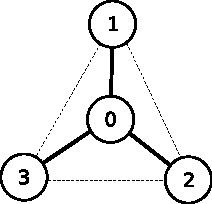
\includegraphics[width=.3\linewidth]{star_config}
\hspace{1cm}
\def\svgwidth{.45\linewidth}
{\footnotesize
\input{img/spectrum.pdf_tex}
}
\caption{The left image sketches the connectivity of our model. The right-hand side displays the energy spectrum in units of $E/J$ for the Star couplings when $n=3$.}
\label{fig:spectrum}
\end{figure}

Now, consider the special configuration of couplings
\begin{align}
 w_{0k} &= 1 \quad \forall \ k  \in \{ 1, \ldots, n \}   && \text{(Star couplings)}  \label{eq:star} \\
 w_{jk} &= 0 \quad \forall \ j \geq 1. \nonumber
\end{align}
This gives rise to a star-shaped connectivity, where all work qubits are coupled to the ancilla, but not among each other. Now, $\Hi$ has a spectrum as indicated in \cref{fig:spectrum}: the ground energy is $E=- J n/2$ when all work qubits are \emph{different} from the ancilla, and $+J$ energy is added for each work qubit that is the same. The complete eigensystem is
\begin{align*}
\{ \ket{0, \vec{x} } : |\vec{x}|_H = \q \}  & & E_{0,\vec{x}}/J = \frac{n}{2}-q && \text{(Star couplings)}  \\
\{ \ket{1, \vec{x} } : |\vec{x}|_H = \q \} & & E_{1,\vec{x}}/J = -\left( \frac{n}{2}-q \right)
\end{align*}
where $|\vec{x}|_H = \q \in \{ 0, \ldots, n \}$ denotes the Hamming weight (i.e. the number of ones) of the bitstring $\vec{x} \in \{ 0, 1 \}^n$. For this configuration, $H_{\vec{x}}$ takes a particularly simple form: the gap $\Delta_{\vec{x}} = J (n-2 \q)$ is the same for all subspaces with the same Hamming weight $\q$, and the mean energy $\bar{E}_{\vec{x}} = 0$ vanishes for all subspaces. 

Now, let us turn on the couplings $w_{jk}$ between the work qubits, leaving the couplings connected to the ancilla fixed at $w_{0k} = 1$. The resulting changes in energy due to $\Hi$ can now only depend on the state $\vec{x}$ of the work qubits, not on the state of the ancilla. Hence, the energy gap $\Delta_{\vec{x}} = E_{0,\vec{x}} - E_{1,\vec{x}}$ will not change as a response to this. In fact, the only parameter of $H_{\vec{x}}$ that changes is $\bar{E}_{\vec{x}}$, leading to a subspace-dependent phase. 

Even more generally, we may \emph{also} allow varying couplings to the ancilla. In this case, the energy gap varies per subspace,
\begin{align}
\Delta_{\vec{x}} = J \sum_{j=1}^n w_{0j} (-1)^{\vec{x}_j},
\end{align}
but does not change $\bar{E}_{\vec{x}}$. In general, this changes each of the $2^n$ subspaces in a different way, making the time evolution even harder to track. 

In the following, we will first assume the most general case, allowing us to obtain exact expressions for the time evolution of any individual subspace $H_{\vec{x}}$. Next, we will resort to certain assumptions that allow us to compute the time evolution of the \emph{full} $2^N$-dimensional system in an efficient way, i.e. requiring a time that scales polynomially with the system size $n$. 




\section{Resonant driving on Ising eigenstates}


We consider two possible driving fields for \cref{eq:hdrive},
\begin{align*}
\alpha(t) &= 2 \Omega \cos(\Dres t + \phi) , \hspace{.35cm} \beta(t) = 0  && \text{single quadrature} \\
\alpha(t) &= \Omega \cos(\Dres t + \phi) , \hspace{.35cm} \beta(t) = \Omega \sin(\Dres t + \phi)   && \text{two quadratures}
\end{align*}
where $\phi$ is the driving phase, and $\Omega$ is the Rabi frequency, which sets the energy scale. Due to the decomposition in \cref{eq:star_decomposition}, the approximation that driving excitations occur in isolated two-level systems that we dicussed in \cref{sec:resdrive} becomes \emph{exact}. For the case of two-quadrature driving, we can analytically solve the evolution of the two-dimensional subsystems, by moving to the rotating frame for each space $\mathcal{H}_{\vec{x}}$. Using the transformation
\begin{align}
U_{\text{int}}(t) = \exp\left( +i t \left( \frac{ \Dres Z }{2} + \bar{E}_{\vec{x}} \mathds{1} \right) \right)
\label{eq:Uint}
\end{align}
the Hamiltonian $H_{\vec{x}}$ becomes time-independent:
\begin{align*}
\tilde{H}_{\vec{x}} & = \begin{pmatrix}
\frac{\Delta_{\vec{x}} - \Dres}{2} & \Omega e^{-i \phi} \\
\Omega e^{i \phi} & - (\frac{\Delta_{\vec{x}} - \Dres}{2})
\end{pmatrix} \\[3mm]
 & = \delta Z + \Omega \left( \cos(\phi) X + \sin(\phi) Y \right).
\end{align*}
We use tildes to indicate that quantities are valid in the rotating frame, and use $\delta$ as shorthand for the off-resonance, $\delta = \frac{\Delta_{\vec{x}} - \Dres}{2}$. Having removed the time-dependence, the unitary effect of $\tilde{H}_{\vec{x}}$ after time $t$ can be calculated as
\begin{align}
\tilde{U}_{\vec{x}}(t) = \exp( -i \tilde{H}_{\vec{x}} t ) = \cos( v t ) \mathds{1} - i \sin( v t ) \frac{ \vec{\sigma} \cdot \vec{v} }{v} \label{eqn:Uq} \\
\vec{v} = \begin{pmatrix}  
\Omega \cos(\phi) \\ \Omega \sin(\phi) \\ \delta 
\end{pmatrix} , \quad v = \sqrt{ \Omega^2 + \delta^2 }, \nonumber
\end{align}
where $\vec{\sigma} = \{ X, Y, Z \}$. Note that $\delta$ is the only parameter that implicitly depends on $\vec{x}$. 

As before, we find selective state inversion. When the subspace labeled $\vec{x}$ is on resonance, i.e. when $\Dres = \Delta_{\vec{x}}$, then a rotation around a vector in the $X-Y$ plane occurs, leading to a perfect inversion at stopping time $T = \frac{\pi}{2 \Omega}$:
\begin{align*}
\tilde{U}_{\vec{x}}(T) = -i (\cos(\phi) X + \sin(\phi) Y ) && \text{(on resonance, } \Dres = \Delta_{\vec{x}}).
\end{align*}
%
%
For off-resonant subspaces, i.e. assuming $| \Omega | \ll |\Dres - \Delta_{\vec{x}} |$, a rotation very close to the non-driven case ($\Omega = 0$) is obtained:
\begin{align}
\tilde{U}_{\vec{x}}(t) \approx \exp \left( -i \delta Z t \right) && \text{(off resonance, }   \Dres \neq \Delta_{\vec{x}} ).
\label{eqn:offres}
\end{align}
We will assess the error introduced by the driving fields compared to the non-driven case shortly. 





\section[Turning the driven evolution into a Toffoli]{Turning the driven evolution into a \texttt{Toffoli}}
\label{sec:circuits}

Let us now assess how the resonant transition is similar to a $\texttt{Toffoli}$ gate. If all $w_{0j}$ are nonzero and have the same sign, then the subspace $\vec{x} = 11\ldots 1$ has the largest or smallest energy gap $\Delta_{\vec{x}}$, which is unique. Choosing $\Dres = \Delta_{\vec{x} = 1 \ldots 1}$, the resulting evolution after time $T$ is then very similar to a \texttt{Toffoli} gate, where the ancilla is flipped if and only if the work qubits are in a state $\ket{1}$. Moving back from the rotating frame to the lab frame using $U_{\vec{x}} = U_\text{int}^\dagger(t) \tilde{ U }_{\vec{x}}$, we obtain the following operation $U_\text{tot}$ at time $T$:
%
\begin{align*}
U_\text{tot} \approx 
\begin{blockarray}{ccccccccc}
  & \text{basis:} &  &   0 \vec{x} & 1 \vec{x} &  & &   0 1\ldots 1 & 1 1\ldots 1 \\
\begin{block}{c(cccccccc)}
  & \ddots &  &  &  &  &  &  &  \\
  &  & \ddots &  &  &  &  &  &  \\
  &  &  & e^{-i E_{{ 0, \vec{x} }} T} & 0 &  &  &  &  \\
  &  &  & 0 & e^{-i E_{{ 1, \vec{x} }} T} &  &  &  &  \\
 &  &  &  &  & \ddots &  &  &  \\
 &  &  &  &  &  & \ddots &  &  \\
 &  &  &  &  &  &  & 0 & -i e^{-i \phi - i E_{ 0, 1\ldots 1} T} \\
 &  &  &  &  &  &  & -i e^{i \phi -i E_{1, 1\ldots 1} T}& 0 \\
\end{block}
\end{blockarray} 
\end{align*}
%
%
%
%
%
%
%
%
%
%
%
%
%
%
%
%
%
%
Even if one accepts the approximation in \cref{eqn:offres}, there are two important differences from an actual \texttt{Toffoli}$_N$ gate:
%
\begin{enumerate}
\item The additional phase $-i e^{\pm i \phi}$ in the resonant subspace $\vec{x}=1\ldots 1$. Note that this is \emph{not} a global phase.
\item The additional phases $E_{x_0,\vec{x}} T$ due to $\Hi$.
\end{enumerate}
%
The $2^N$ different energies $E_{x_0,\vec{x}}$ can in general be hard to compute for a large system. Undoing them may be even harder. However, one can conceive various specific configurations where resetting the phases is possible.

In particular, whenever the system is symmetric under permutations on the work qubits, then all subspaces with the same Hamming weight $q$ behave the same, and only $n+1$ different subsystems have to be considered. Various techniques can then be used to undo the dynamical phases. One example is to choose a total gate time $T$ such that all phases are $E_{x_0,\vec{x}} T$ become a multiple of $2\pi$. For example, in the star configuration, the energy differences are all integer multiples of $J$, hence choosing a total driving time $T = 2 k \pi / J \ (k \in \mathbb{N})$ gets rid of unwanted phases. 


%
%
%
Assuming we have somehow removed the phases due to $\Hi$, we turn to removing the phases $-i e^{\pm i \phi}$, for which we propose the circuit below:
%
\begin{align}
\Qcircuit @C=1 em @R=.6 em {
 & \ctrl{1} & \qw & \raisebox{-6.3 em}{=} & & \qw & \qw & \multigate{5}{{U_\text{tot}}} & \qw &  \multigate{5}{{ U_\text{tot}}} & \qw & \qw & \qw \\
 & \ctrl{1} & \qw &                       & & \qw & \qw & \ghost{{\rm U_\text{tot}}} 		& \qw & \ghost{{\rm U_\text{tot}}} 		& \qw & \qw & \qw \\
 & \ctrl{1} & \qw &                       & & \qw & \qw & \ghost{{\rm U_\text{tot}}} 		& \qw & \ghost{{\rm U_\text{tot}}}		& \qw &  \qw & \qw \\
 & \ctrl{1} & \qw &                       & & \qw & \qw & \ghost{{\rm U_\text{tot}}} 		& \qw & \ghost{{\rm U_\text{tot}}} 		& \qw & \qw & \qw  \\
 & \targ 	& \qw &                       & & \gate{H} & \qw & \ghost{{\rm U_\text{tot}}}  	& \qw & \ghost{{\rm U_\text{tot}}}		& \qw & \gate{H} & \qw \\
 &                &      				  & & 	  & 	& \lstick{\ket{0}} & \ghost{{\rm U_\text{tot}}} & \qw & \ghost{{\rm U_\text{tot}}} & \qw & \lstick{{\ket{0}}} \\
}
\label{eq:circuit}
\end{align}
%
Note that applying the resonant operation \emph{twice}, leads to a phase $-1$ in the resonant subspace. This is similar to a multiple-controlled $Z$ gate except that the sign is applied both when the ancilla is in state $\ket{0}$ and when it is in state $\ket{1}$. Hence, we obtain a multiple-controlled $Z$-gate which applies a sign $-1$ to the work qubits if and only if all these qubits are in the state $\ket{1}$. The state of the ancilla is unimportant, and we may just as well initialize it to $\ket{0}$ before the protocol. Finally, the controlled-$Z$ is mapped to a controlled-$X$ by using two Hadamard gates -- these can be applied to any work qubit, and that qubit then takes the role of target of the \texttt{Toffoli}$_n$.




\subsection{Expressing the gate error}
We turn back to \cref{eqn:offres}, which we claim is a good approximation to the off-resonant evolution stated in \cref{eqn:Uq}. To assess the quality of this approximation, we consider two different measures of gate error. Firstly, the \emph{trace error} or \emph{matrix inner product} is defined as
\begin{align*}
\mathcal{E}_\text{tr} (U, U_\text{goal}) = 1 - \frac{1}{\text{dim}(U)} \text{tr}( U U_\text{goal}^\dagger )
\end{align*}
which gives an averaged error. Secondly, the \emph{operator norm} of the difference is given by 
\begin{align*}
\mathcal{E}_\text{norm}(U, U_\text{goal}) = || U - U_\text{goal} ||
\end{align*}
which returns the largest eigenvalue of $U - U_\text{goal}$ and hence captures the worst-case error of our gate. 

Let us now assume a permutation symmetry among the work qubits. Then the evolution $\tilde{U}_{\vec{x}}$ depends only on the Hamming weight $q$ of the vector $\vec{x}$, and we will use $U_q$ to denote the evolution in subspaces with $|\vec{x}|_H = q$. We can then simplify the expressions for the gate error. For the matrix inner product,
\begin{align*}
\mathcal{E}_\text{tr} (U, U_\text{goal}) = 1 - \frac{1}{\text{dim}(U)}  \sum_{q=0}^n \text{tr}( U_q  U_{\text{goal},q}^\dagger ) { n \choose q }
\end{align*}
where the binomial coefficient counts the number of subspaces with the corresponding Hamming weight. Likewise, 
%
\begin{align*}
\mathcal{E}_\text{norm}(U, U_\text{goal}) = \max_q || U_q - U_\text{goal,q} ||.
\end{align*}

In the following, we choose to work in the interaction picture, as defined by \cref{eq:Uint}. This way, the energies $E_{x_0, \vec{x}}$ due to $\Hi$ drop out, allowing us to assess purely the driving error at any gate time $T$. Then, the work qubits need not even be completely permutation symmetric: assuming identical couplings to the ancilla is sufficient to justify a $q$-dependent treatment. Still, to obtain a proper quantum gate, the dynamical phases need to be undone somehow. 

To form a resonant gate, we choose the driving frequency $\Dres$ to be resonant with the subspace with weight $q_0 = 0$, i.e. $\Dres = \Delta_{\vec{x} = 0\ldots 0}$. Note that his is equivalent to the case $q_0=n$ of the \texttt{Toffoli} gate we considered before, but will lead to slightly cleaner notation. We stress that other configurations  and other resonant frequencies $\Dres$ can be addressed analogously. 

We choose to keep $T$ as a free parameter, such that the errors will become a function of the total gate time. Setting $\Omega = \frac{\pi}{2T}$ guarantees that for any $T$, a perfect inversion occurs in the resonant subspace. The evolution in the resonant subspace $q=0$ is always exact (no error), while the off-resonant evolutions $\tilde{U}_q$ for $q \neq 0$ are compared to the goal $\tilde{U}_\text{goal,q} = e^{-i \delta Z t}$, with $\delta = -Jq$ for the star couplings.
%


For the trace inner product, we obtain fidelities for subspaces $q$ as
\begin{align*}
\mathcal{F}_q := \text{tr} \left(  \tilde{U}_q(T) \tilde{U}^\dagger_\text{goal,q}(T) \right) &= 2 \cos( J T q ) \cos(J T \nu) +  \frac{2q}{\nu}  \sin( J T q) \sin( J T \nu ) \\
\text{ with } \nu &=  \sqrt{\frac{\pi}{4 J^2 T^2} + q^2} 
\end{align*}
In \cref{fig:Etrace}, we plot the dependence of $\mathcal{F}_q$ as a function of gate `time' $J T$, as well as the average error $\mathcal{E}_\text{tr}$ for varying $n$. We find that according to this metric, the gate fidelity actually \emph{improves} with larger system sizes, which is explained as follows. For any $n$, there are $n$ subspaces with weight $q=1$ which are the least off-resonant, but an exponentially large number of subspaces with much larger off-resonance are added. Hence, the averaged error benefits more from the many off-resonant subsystems when $n$ increases.

\begin{figure}
\centering
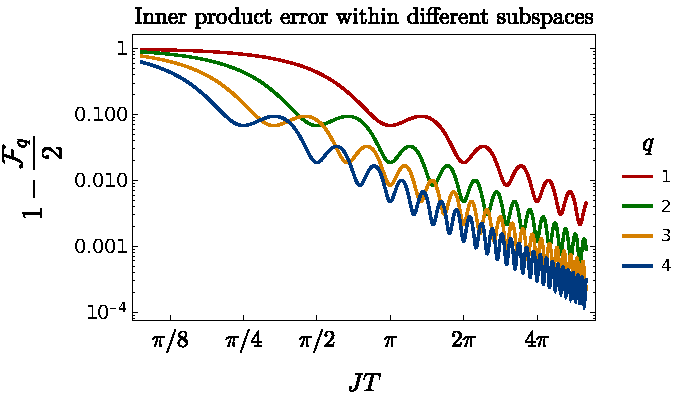
\includegraphics[width=.67\textwidth]{img/EtrVsW} \\
\hspace{.73cm} 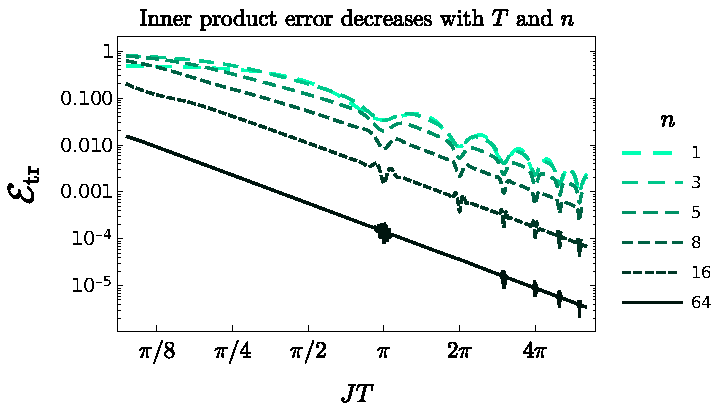
\includegraphics[width=.7\textwidth]{img/EtrVsTandN}
\caption{The inner product error as a function of gate time $T$, assuming the resonant subspace has weight $q_0 = 0$. Note that the vertical axes follow a logarithmic scale. Top: The error contribution for subspaces whose weights differ from $q_0$ by $1$ up to $4$. Bottom: The cumulative error $\mathcal{E}_\text{tr}$, for various system sizes $n$. }
\label{fig:Etrace}
\end{figure}


For the operator norm, we obtain 
\begin{align*}
\tilde{U}_q(T) - \tilde{U}_{\text{goal},q}(T) = & \ \mathds{1} \left( \cos( J T \nu ) - \cos(J T q) \right) \\
& + Z \left( \frac{iw}{\nu} \sin( J T \nu ) - i \sin(J T q) \right) \\
& + (\cos(\phi) X + \sin(\phi) Y ) \left( \frac{-i \pi}{2 J T \nu} \sin(J T \nu) \right),
\end{align*}
allowing us to efficiently calculate the exact operator norm error in each individual weight-$q$ subspace. The results are shown in \cref{fig:Enorm}. It is clear that the most resonant subspace, $q=1$, always contributes the largest error. Therefore, the $\max$ operation can be dropped in $\mathcal{E}_\text{norm}$, and we find that operator norm error is actually \emph{independent} of $n$. 

\begin{figure}
\centering
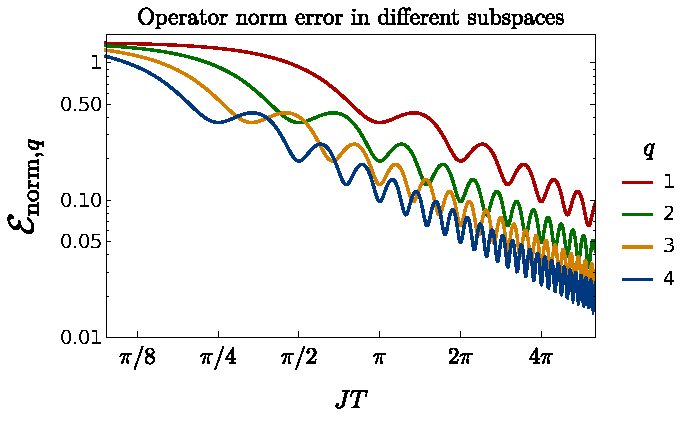
\includegraphics[width=.67\textwidth]{img/EnormVsW}
\caption{The operator norm error $\mathcal{E}_{\text{norm},q}$ contributions due to subspaces with weights $q=1, \ldots 4$, at various protocol times. The overall error $\mathcal{E}_\text{norm}$ for the whole gate is always the maximum, hence is completely determined by $q=1$. }
\label{fig:Enorm}
\end{figure}



The same derivation could be performed whenever a subspace different from $q_0=0$ is to be flipped. By choosing the driving frequency $\Delta= J (n-2q_0)$, one will approximately find the operation where ancilla is inverted if and only if the work qubits have weights $|\vec{x}|_H = q_0$. The values $q$ in the above should then be replaced with $q-q_0$. 

Lastly, we consider the effect of using single-quadrature driving instead of the two-quadrature driving fields we consider above. Hence, we assume that 
\begin{align*}
\alpha(t) \propto \cos(\Dres t) \propto \exp(i \Dres t) + \exp(- i \Dres t)
\end{align*} 
such that effectively \emph{two} driving fields act on each two-dimensional subspace. The two resonant resonant energies differ by a sign namely $\Dres$ and $-\Dres$. Assuming that $\Hi$ is the only Hamiltonian that acts on the qubits, then $\Delta_{\vec{x} = 1 \ldots 1} = - \Delta_{\vec{x} = 0 \ldots 0}$. This voids our argument that the subspace labeled $\vec{x} = 11\ldots 1$ is the unique resonant subspace, because $\vec{x} = 00\ldots 0$ is now also on resonance. 

\sloppy{There are two straightforward solutions that prevent the transition $\ket{0,0\ldots 0} \leftrightarrow \ket{1, 0 \ldots 0}$ from taking place.} We can do so by turning one work qubit into an ancilla that is initialized to the state $\ket{1}$, such that the $\vec{x} = 0\ldots 0$ subspace is never populated. The other solution is to consider a local field of the form $H = B Z_0 / 2$ acting on the ancilla qubit, with some field strength $B$. The relevant energy gaps are then $B + \Delta_{\vec{x} = 1 \ldots 1}$ and $B - \Delta_{\vec{x} = 1 \ldots 1}$, which no longer differ by a sign. Most experimental quantum computers already feature some energy difference between the $\ket{0}$ and $\ket{1}$ state, making the second solution a very natural choice. 

Moreover, note that under single-quadrature driving, our results are no longer exact. Still, the Rotating Wave Approximation (RWA) shows that our reasoning about resonant and off-resonant subspaces still holds as long as detunings are large compared to other energy scales.


\section{Discussion of asymptotic scaling}
In the above, we assumed that $n$ qubits were strongly coupled to our ancilla, and that the \emph{driving frequency $\Dres$} has no bounds. Then, the protocol time and the errors are roughly \emph{constant} as a function of $n$. This is surprising, as this is a better asumptotic scaling than the $O(\log(n))$ time required by a gate-based quantum circuit. In particular, in our proposals in \cref{chap:krawtchouk,chap:pc}, the gate time increased \emph{superpolynomially} with $n$. 

Still, it is not immediately clear if our assumptions are realistic. Firstly, the oscillation frequency $\Dres$ for the resonant subspace $q_0 = n$ increases linearly with $n$ in our protocol. This may not be realistic, and if one requires the frequency $\Dres$ to be bounded, then the Hamiltonian's energy scale needs to be scaled down with a factor $1/n$. This effectively causes all time scales to increase by a factor $n$, retrieving an $O(n)$ time protocol. 

Secondly, coupling $n$ qubits to a single ancilla would be challenging to realize in physical, 3-dimensional space, as each of these $n$ qubits would need to be sufficiently close to the ancilla.  Any realistic method to implement this would probably set a maximum for $n$. 


\section{Experimental implementations}
We consider two experimental platforms on which our proposal could be implemented in near-term experiments. Firstly, ultracold atoms of the Rydberg type natively feature a strong Ising-type interaction \cite{Saffman2016}. Various earlier proposals for multiqubit operations based on the Rydberg blockade interaction exist, such as Refs. \cite{Lukin2001,Unanyan2002,Isenhower2011,Shi2018}, and some of these have been experimentally tested \cite{Ebert2015,Zeiher2015}. The specific \texttt{Toffoli}-type gates have, to our best knowledge, never been implemented, but Ref. \cite{Gulliksen2015} performs a detailed simulation of the \texttt{Toffoli}$_3$ proposed in Ref. \cite{Isenhower2011}, finding that the multiqubit implementation may have advantages over a sequence of one- and two-qubit gates. 

Secondly, trapped ions are very well suited to simulate the Ising model with all-to-all connectivity. These systems typically involve ionized atoms positioned on a line, and for each ion, two electronic states are chosen to form the qubit degree of freedom. By coupling the qubits to motional states of the ions using a two Raman lasers, an effective interaction between the qubits can be formed, which approximates the Ising model. The couplings strengths are then of the form $w_{jk} \propto 1 / ( j - k )^\alpha$ with $\alpha \in [0,3]$ \cite{Kim2009,Blatt2012,Britton2012,Islam2013}. The choice $\alpha=0$ makes all interactions equal, leading to a highly symmetric system for which the energies $\bar{E}_{\vec{x}}$ are efficiently calculated. 

We identify various challenges for a real-world implementation of our gate using trapped ions. Firstly, the amplitude of the Ising interaction $J$ is determined by the off-resonance between the Raman lasers and a certain transition in which a phonon is created. Entanglement with phonons can be avoided by choosing a sufficiently large detuning, which in turn leads to a small interaction strength $J$. Because our resonant field on the ancilla must have an amplitude $\Omega$ that is much smaller than $J$, there are two mechanics at play that favor a very small value of $\Omega$, leading to very long gate times for an accurate gate. Alternatively, choosing the Raman lasers closer to resonance with the relevant transition increases $J$, but causes the phonon number to oscillate with larger amplitude. Driving a transition between the states $\ket{1,\vec{x}}$ and $\ket{0,\vec{x}}$ when these are entangled to a different phonon number introduces unwanted errors in the final gate. Therefore, a competitive implementation of our proposal on trapped ions requires further optimization. 

To illustrate, a closely related experiment was performed in Ref. \cite{Senko2014}. Here, up to 18 ions are made to approximate some Ising interaction, while at the same time, a resonant driving field is applied to \emph{all} ions simultaneously. The interaction strength is of the order of a few kHz, which is sufficiently strong to identify certain transitions for spectroscopic applications. However, we believe that the resulting evolution is too inaccurate to form a high-fidelity multiqubit gate at this point.


\section{Conclusion}
In conclusion, we studied resonant driving on an ancilla qubit coupled to $n$ other qubits through Ising interactions, and find that a highly selective operation can be obtained, namely a a bitlip if and only if the work qubits have a certain Hamming weight. The Hamiltonian block-diagonalizes into invariant two-dimensional subspaces, and if the energies of each subspaces are known, then we can efficiently track the state's evolution within that space. This allows us to calculate exact values of the error compared to an ideal \texttt{Toffoli}$_n$ gate. The gate time, at constant error, is found to be a non-increasing function of the system size, under the assumption that interaction strengths remain constant and that the driving field can oscillate at arbitrary frequencies. For near-term quantum computers of moderate system size, this approach could lead to fast and high-precision multiqubit gates. 